\documentclass[nofoot]{asmeconf}
\usepackage{graphicx,booktabs}
\ConfName{Proceedings of the ASME 2027\\International Design Engineering Technical Conferences and\\Computers and Information in Engineering Conference}
\ConfAcronym{IDETC/CIE2027}
\ConfDate{August 1--4, 2027}
\ConfCity{Philadelphia, PA}
\PaperNo{}
\title{Separating Buoy Registration Error and Echo Loss Under Wave-Driven Vessel Motion}
\SetAuthors{J.C. Vaught\affil{1}}
\SetAffiliation{1}{University of South Carolina, Columbia, SC}
\begin{document}
\maketitle
\begin{abstract}
A buoy track can lose an update when an echo fades or when vessel motion moves its mapped position outside tolerance. We cross antenna pointing and registration time on identical wave-driven visits to determine how much each intervention recovers on its own and after the other is installed. Treating echo survival and position error as independent overestimated the gain from registration by up to 9.11 percentage points. In one simulated condition, leveling alone gained 24.01 percentage points in usable positions. After spoke-time registration was installed, the same hardware gained only 0.85 points. Most of its stand-alone benefit came from relocating echoes that both antennas received. Across 111 regular-wave conditions with prescribed range and bearing errors, replacing a 625 ms pose delay with exact timing gained a median 3.37 points at a 0.50 m tolerance. Replacing a 50 ms delay gained only 0.07 points. On two recorded 4 Hz vessel-radar clips, median repeat separation of matched returns improved by 6 mm and less than 1 mm. In simulations of revisit timing, a frequency-based selector never beat fixed 48 rpm across 40 held-out conditions. The value of a retrofit therefore depends on how the existing radar timestamps returns, which echoes survive, and which correction is already installed.
\keywords{forced vibration, marine radar, vessel motion, wave diffraction, scan registration}
\end{abstract}

\section{Introduction}
A tracker on a small vessel can miss a buoy position because a crest attenuates the echo or because the assigned pose puts a surviving echo outside tolerance. Both events depend on wave phase. Estimating their rates independently can therefore misstate how many positions a timestamp correction would recover. A stabilized mount complicates the choice further because it can change the location assigned to an existing echo as well as the power available during acquisition.

We ask whether a designer should change the timestamp, the pointing, or the scan period. A four-arm comparison measures each retrofit alone and after the other is installed on the same scheduled visits. We test a separable model of echo and position losses, measure sensitivity to hull damping and propagation, and compare two timestamp policies on recorded radar returns. The denominator is all attempted visits. Track continuity is evaluated separately over equal elapsed time.

\section{Related work}
\label{sec:related-work}

\subsection{Shipboard registration and antenna pointing}

Shipboard marine radar already uses acquisition-time navigation data when motion within a rotation matters. McCann and Bell calibrated azimuth, range, and timing offsets by maximizing the sharpness of shipborne X-band images accumulated using timestamped radar and navigation data \cite{McCann2018OffsetCalibration}. Lund et al. interpolated position and heading to individual radar pulses for sea-ice drift retrieval and treated heave, pitch, and roll as smaller than the 7.5 m range resolution for their application \cite{Lund2018SeaIceDrift}. Hessner et al. likewise georeferenced pulses with time-matched navigation data and relied on the broad elevation beam of the radar aboard \emph{Polarstern} to accommodate its typical pitch and roll \cite{Hessner2019Reliability}. On vessels under 15 m, Simpson et al. aligned radar-derived wave fields using wave and buoy signatures and identified antenna-height variation as a possible source of amplitude error \cite{Simpson2020Forecasting}. Together, these studies establish pulse-time registration and show that the importance of vertical motion depends on the measurement scale and platform.

Burnett et al. measured the effect of compensating motion distortion on spinning-radar navigation \cite{Burnett2021MotionDistortion}. Chen et al. showed how time-varying attitude affects the observability of position and attitude biases for mobile radar \cite{Chen2014Registration}. Xie et al. studied vertical motion of shipborne X-band radar in significant-wave-height estimation \cite{Xie2019WaveCompensation}. These studies evaluate navigation, registration, or wave retrieval. Here the design quantity is the change in the number of attempted buoy visits that yield an accurate position when pointing, timestamp, or both are changed.

In coastal radar odometry, Jang et al. improved estimates of vessel rotation by matching successive radar images with maritime scene features \cite{Jang2024MaritimeOdometry}. That correction acts on recorded data. By comparison, Mar et al. evaluated ship-motion compensation that changes the direction of a phased-array beam toward an airborne target \cite{Mar2013Motion}. A rotating radar observing a buoy likewise couples registration and illumination to the same vessel motion, but the two interventions enter at different stages. Registration changes the position assigned to an acquired echo. Pointing changes the signal available to the detector during the visit.

\subsection{Crest clearance and low-elevation target returns}

Studies of marine radar imaging show why the direct ray alone cannot predict received power. Wijaya and van Groesen used geometric shadowing to generate synthetic sea-surface radar images for wave-height retrieval \cite{Wijaya2016Shadowing}. In measurements of deep-water ocean backscatter, Plant and Farquharson found that geometric shadowing poorly described low-grazing-angle dropouts \cite{Plant2012WaveShadowing}. Janssen et al. calculated X-band diffraction around smooth wave crests and found finite illumination within nominal ray shadows and reduced illumination immediately outside them \cite{Janssen2026Diffraction}. Their calculation treats incident illumination of the water surface. A buoy echo also depends on scattering from the target and propagation back to the receiver.

Herselman et al. measured calibrated X-band returns from small craft at medium-to-low grazing angles. Small-boat echoes faded as the craft entered wave troughs, and the return from a boat heading into the waves showed periodicity at the mean wave period \cite{Herselman2008SmallBoat}. Those measurements connect wave phase to the strength of a low-elevation target echo. They also identify multipath and clutter as contributors to variability. Clutter-adaptive radar detectors estimate the local background to set a threshold \cite{Rohling1983RadarCFAR}. Thus a prescribed clear-path margin can isolate the effects of obstruction and pointing, while estimates of detection probability for a particular radar and buoy require measured target and clutter returns.

\subsection{Wave shape and vessel response}

The crest and vessel attitude share the same wave forcing, but their relative phase depends on the hull response. Mounet et al. fitted wave-to-motion transfer functions to inertial data from an AutoNaut unmanned surface vessel. The estimated heave and pitch spectra agreed more closely with measurements than the roll spectra did, even after calibration \cite{Mounet2024Hydrodynamic}. Crest shape introduces a separate effect. Second-order wave interactions sharpen crests and change their height distribution \cite{Tayfun1980Nonlinear,Forristall2000Crest}. McAllister and van den Bremer measured distinct second-order motions for a surface-following buoy and a fixed wave gauge in the same steep wave groups \cite{McAllister2019Lagrangian}. These results motivate treating hull response, intervening crest shape, and buoy motion as separate inputs to path clearance.

The present comparison links these inputs over the same scheduled visits. Processing the same echo with two poses measures the mapping penalty due to the scan timestamp. Recomputing acquisition with level pointing reveals which visits cross the echo threshold when the antenna changes attitude. Counting consecutive failures tests the influence of scan timing on the gaps between usable positions.


\begin{figure*}[t]
\centering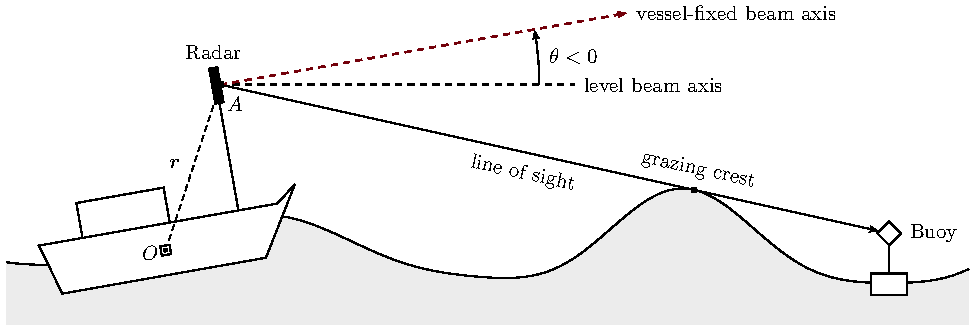
\includegraphics[width=.94\textwidth]{figures/operating/geometry.pdf}
\caption{Radar and buoy geometry. The bow-up attitude has negative pitch. The lever from pivot $O$ to antenna phase center $A$ runs forward and upward in body coordinates. The level and vessel-fixed axes pass through the same displaced antenna origin. The path clearance depends on the instantaneous elevations of both endpoints and of the intervening water.}
\label{fig:geometry}
\end{figure*}

\section{Wave forcing and vessel response}
Let $x$ point along the nominal bow and $z$ upward. The nominal buoy location is $(100,0)$ m in the horizontal plane. For a deep-water component with amplitude $a$, frequency $f$, direction $\gamma$, and initial phase $\psi$, the surface elevation follows from the dispersion relation \cite{MITOCW2005LinearWaves},
\begin{equation}
 \eta(\mathbf{x},t)=a\cos(\mathbf{k}\cdot\mathbf{x}-\omega t+\psi),
 \quad k=\omega^2/g,\quad \omega=2\pi f .
\end{equation}
Here $\mathbf{k}=k(\cos\gamma,\sin\gamma)$ and $g=9.81$ m/s$^2$. The vessel has zero mean forward speed. Consequently, the nominal encounter frequency equals the wave frequency. Each component drives the hull at its mean location. The instantaneous radar and buoy positions enter the subsequent obstruction calculation.

For the baseline hull model, the pitch angle $\theta$ is positive bow down. The pitch mode follows the longitudinal slope with prescribed static gain $G=0.25$. With damping ratio $\zeta$, natural frequency $f_n$, and $\omega_n=2\pi f_n$, its forced equation and steady-state response factor are
\begin{align}
 \ddot\theta+2\zeta\omega_n\dot\theta+\omega_n^2\theta
 &=-\omega_n^2G\,\partial_x\eta(\mathbf{0},t),\\
 H(r,\zeta)&=(1-r^2+2\mathrm{i}\zeta r)^{-1},\quad r=f/f_n .
\end{align}
Thus peak pitch is $Gka\cos\gamma\,|H|$. To reproduce the other degrees of freedom, let $q=\exp[\mathrm{i}(\omega t-\psi)]$ and take the real part of each expression. Pitch is $\mathrm{i}Gka\cos\gamma\,Hq$, roll is $0.6Gka\sin\gamma\,Hq\exp(\mathrm{i}\pi/3)$, and the prescribed surge proxy is $\mathrm{i}a\cos\gamma\,q$. Heave is $aH(f/0.80,0.30)q$. Linear superposition gives the irregular-wave response. These coefficients prescribe a reproducible hull response. Measured response spectra depend on hull, loading, and encounter conditions, as demonstrated for the AutoNaut by Mounet et al. \cite{Mounet2024Hydrodynamic}.

The still-water hull reference point is $(0,0,1.20)$ m. The 100 m target distance is measured from its horizontal projection, placing the forward target 99.4 m horizontally from the still-water antenna. The body rotation is $Q=R_y(\theta)R_x(\phi)$, where $\phi$ is roll. Applying it to the antenna lever arm $(0.6,0,0.8)$ m and adding surge and heave gives the antenna origin $\mathbf{o}$. The buoy remains horizontally fixed and its scattering point follows the local water level at a fixed offset. Figure~\ref{fig:geometry} shows why leveling the antenna changes pointing without moving either endpoint of the propagation path.



\section{Acquisition and registration}
The Furuno DRS4D-NXT provides a documented rotation period and vertical beamwidth for the study \cite{Furuno2016DRS4DNXT}. Table~\ref{tab:inputs} distinguishes those specifications from the modeled conditions. Let $\beta$ be the full one-way half-power beamwidth and $e$ the buoy elevation in the antenna frame. A Gaussian power pattern on both transmit and receive gives two-way angular loss
\begin{equation}
 L(e)=80\log_{10}(2)(e/\beta)^2\quad \text{dB}.
\end{equation}
The nominal radar wavelength approximates the X-band carrier. The 10 dB boresight margin is a control on proximity to the detector threshold. Range, freeboard, lever arm, 25-degree heading, and the modal gains define a test geometry and vessel, without a fitted sea trial. The 0.35 Hz natural frequency places a resonance within the wave-frequency sweep. We vary damping, wave amplitude, and echo margin so that results depending on those choices can be identified. With this convention, the two-way loss at $|e|=\beta/2$ is 6.02 dB. For the vessel-fixed case $e$ comes from the true line of sight expressed in the moving body frame. The level case uses elevation above a horizontal plane through the same origin.

\begin{table}[tb]
\caption{Reference inputs. The manufacturer specifies the first two entries. All remaining values are study assumptions.}\label{tab:inputs}
\centering\small
\begin{tabular}{@{}ll@{}}\toprule
Quantity & Value \\ \midrule
Full vertical beamwidth & $25^\circ$ \\
Rotation period at fixed 24 rpm & 2.5 s \\
Nominal radar height / buoy freeboard & 2.00 / 0.22 m \\
Nominal buoy range / wavelength & 100 / 0.03 m \\
Wave propagation angle to bow & $25^\circ$ \\
Pitch natural frequency / damping & 0.35 Hz / 0.15 \\
Reference wave frequency / amplitude & 0.35 Hz / 0.15 m \\
Clear boresight margin & 10 dB \\
Horizontal error tolerance & 0.50 m \\
\bottomrule\end{tabular}
\end{table}

Wave shadowing can alter low-grazing-angle marine radar returns \cite{Plant2012WaveShadowing}. To represent this effect with an explicit threshold, we approximate the water profile by its most obstructive effective knife edge \cite{ITUR2025P526}. Along the direct ray of slant length $\rho$, let $s$ be the fractional distance from the antenna and let $d(s)$ be water height above the ray. With wavelength $\lambda$, the normalized obstruction is
\begin{equation}
 \nu=\max_{0<s<1}\ d(s)\sqrt{2/[\lambda\rho s(1-s)]}.
\end{equation}
For $\nu>-0.78$, put $u=\nu-0.1$ and set one-way loss $J=6.9+20\log_{10}(\sqrt{1+u^2}+u)$ dB, floored at zero. Otherwise $J=0$. With clear boresight margin $M_0$, the echo is acquired when $L(e)\le h$, where $h=M_0-2J$. This deterministic model fixes the clear-path margin and omits clutter, multipath, target scintillation, and range-dependent spreading over the small range excursions considered here.

This inequality identifies the visits that leveling can recover. Recovery requires $L(e_{\rm level})\le h<L(e_{\rm body})$. If $h<0$, even zero pointing loss cannot produce an echo. A tilted beam can also point closer to the buoy, in which case leveling can lose a visit. With no diffraction and 10 dB margin the limiting offset is $16.1^\circ$. At the reference wave, summing conservative bounds on heave, buoy height, and lever motion gives $|e_{\rm level}|\le1.26^\circ$. The combined pitch and roll tilt is bounded by $3.33^\circ$. The resulting body pointing loss is at most 0.81 dB, so a reference miss caused by pointing requires more than 9.19 dB of two-way diffraction. A measurement of pitch alone does not identify these near-threshold visits.

For an acquired return, mapping uses slant range $\rho$, antenna-frame azimuth $\alpha$, and the assumed scattering-point elevation $z_T$. Define $\mathbf{a}=Q(\cos\alpha,\sin\alpha,0)^\mathsf{T}$ and $\mathbf{b}=Q(0,0,1)^\mathsf{T}$. The near-horizontal solution for elevation $\epsilon$ and mapped position $\hat{\mathbf{x}}$ satisfies
\begin{align}
 (z_T-o_z)/\rho &= a_z\cos\epsilon+b_z\sin\epsilon,\\
 \hat{\mathbf{x}} &= \mathbf{o}+\rho(\mathbf{a}\cos\epsilon+\mathbf{b}\sin\epsilon).
\end{align}
With known $z_T$, the horizontal range from the assigned origin is $[\rho^2-(z_T-o_z)^2]^{1/2}$. For a forward target with zero roll and yaw and an exact origin, a pure pitch error leaves the reconstructed ray in the same vertical plane. The present geometry therefore gives horizontal errors through origin displacement and coupled attitude, and need not describe a side-looking target or a turning vessel. A midpoint pose represents an entire rotation by a single timestamp, as might be available in an assembled scan. It serves here as a controlled timing error. Existing pulse-timestamped systems can instead be evaluated against their measured latency. The midpoint estimate uses $Q$ and $\mathbf{o}$ at the scan midpoint. The per-spoke estimate uses the same measured return and both quantities at the spoke time. Ideal level pointing recalculates acquisition and azimuth in a level frame at that time. The fourth arm applies a midpoint origin to the level-pointed echo. Its horizontal axes remain level at both times. All four arms share wave phase and visit times. The base case supplies exact range, bearing, and instantaneous target elevation, so residual per-spoke mapping error is zero to numerical precision. This isolates the motion contribution to the 0.50 m tolerance. At 100 m a one-degree bearing error corresponds to 1.75 m cross-range, and the manual quotes bearing accuracy of $\pm1^\circ$ \cite{Furuno2016DRS4DNXT}.

\subsection{What a pose delay changes}
A time error acts on position and attitude together. For a single component, write a pose coordinate as $x(t)=X\cos(\omega t+\varphi)$. Applying the pose from $t-\tau$ gives the following peak coordinate mismatch over one cycle,
\begin{equation}
 \max_t |x(t)-x(t-\tau)|=2|X\sin(\pi f\tau)|.
 \label{eq:pose-delay}
\end{equation}
For short delays the mismatch grows approximately as $2\pi f|X|\tau$. The factor $X$ includes the mechanical frequency response for pitch, roll, and heave. The second factor depends on the timing of the radar measurement. Thus equal peak pitch does not imply equal attitude mismatch at a given delay. Equation~\eqref{eq:pose-delay} bounds an individual coordinate. Horizontal position error also depends on the lever arm, the viewing direction, and the phases at which an echo survives. We therefore evaluate registration with the full inverse geometry on the actual set of acquired spokes.

\section{Paired experimental design}
Each rotation schedules one visit a quarter-turn after the scan midpoint. Keeping visit times fixed pairs the interventions and neglects the change in crossing time as the target bearing moves. Every scheduled visit enters the denominator. A visit either falls below the echo threshold, yields a position outside tolerance, or yields a usable update. We measure both the usable fraction and the longest elapsed gap within a common observation window.

Regular-wave states and rigid-body pose are evaluated analytically at each visit. The production ray calculation uses 601 equal path subdivisions with the endpoints excluded. The operating map samples 17 equally spaced frequencies from 0.16 to 0.62 Hz and 11 amplitudes from 0.04 to 0.60 m. Filtering out $ka>0.20$ or pitch or roll exceeding $10^\circ$ leaves 111 combinations. At this gain, damping, and heading the slope cap alone limits the linear peak pitch to less than $8.8^\circ$. The angle cap removes no additional cells. Each combination uses 32 independently seeded initial wave phases with 192 scheduled visits per phase. Initial phases use a base seed of 5742026. Common phase draws pair the processing cases. A reported random-phase interval uses the paired differences for the 32 realizations, with half-width $1.96$ times their sample standard deviation divided by $\sqrt{32}$. This measures phase-sampling uncertainty in the modeled mean. Adjacent visits share wave dynamics and do not provide independent replicates.

For the timing comparison we prescribe $3^\circ$ peak pitch at 0.20, 0.28, 0.35, and 0.42 Hz by changing wave amplitude. Separate controls shift pitch phase at fixed wave amplitude or distribute the reference elevation variance among seven components on the same heading. The component weights and phases are available with the simulation.

\section{Numerical verification}
Direct integration of the forced pitch oscillator from rest reproduced the analytical response across 19 frequency ratios. Fitting the cycle after 60 periods gave maximum relative amplitude error $5.50\times10^{-12}$ and absolute phase error $3.47\times10^{-10}$ degrees. An independent intersection of the bearing plane and range circle reproduced the inverse mapping within $6\times10^{-14}$ m in three wave conditions. Halving the angular power at half beamwidth produced the expected 6.021 dB two-way loss.

Refining the path from 601 to 2,401 subdivisions changed the modeled margin by at most 0.0211 dB at three test cells and preserved their classifications. At the two cells with negative leveling gains, refinement to 4,801 subdivisions changed individual decisions near threshold. Across four resolutions the gains remained negative, from $-0.31$ to $-0.26$ and $-1.06$ to $-0.90$ percentage points, respectively. Uniformly sampling 32 versus 256 starting phases changed mean usability by at most 3.13 points in the matched-pitch comparisons. The repository provides the convergence data and oscillator response figure.

\subsection{Comparison with a field-fitted pitch response}

Mounet et al.'s field-fitted pitch-amplitude response for a 5 m AutoNaut \cite{Mounet2024Hydrodynamic} gives $3.47^\circ$ at the reference wave and $9.21^\circ$ at the largest registration-gain wave, compared with $3.20^\circ$ and $8.28^\circ$ for the prescribed oscillator. This check uses the published weighted-average parameters at zero forward speed and a $25^\circ$ heading. The spectral fit constrains magnitude but leaves pitch phase relative to a passing crest unresolved.

\subsection{Bounding a pointing benefit from measured margins}
A small change in angular loss can recover only visits sufficiently close to threshold. Let $m_i$ be the measured body-pointed power margin on scheduled visit $i$. If leveling can increase this margin by at most $b$ dB, the net improvement in acquisition fraction is bounded above by
\begin{equation}
 U_b=N^{-1}\sum_{i=1}^N \mathbf{1}\{-b\le m_i<0\}.
\end{equation}
The bound counts every potentially recoverable visit. Losses on previously acquired visits can only lower the net gain. Its application requires comparable margins on all attempts, including misses.

We evaluated the bound on all 14 Dartmouth IPIX weak-target records in the published catalog \cite{McMaster1993IPIX}. Each 9.39 GHz record used a shore-mounted radar at 30 m height and a 1 m wire-wrapped sphere at nominal ranges of 2.66--5.58 km (nominal grazing angles about $0.31$--$0.65^\circ$). We estimated each record's receiver correction and power normalization from clutter in its first quarter, excluding all catalog target bins. A 99th-percentile development-clutter gate yielded 0.41--3.40\% crossings on held-out clutter. Across records, 34.2--97.9\% of the 1,536 held-out primary-bin power windows per record fell below threshold.

Adding 0.81 dB, the reference simulation's upper bound on angular loss, could recover 1.11--4.75 percentage points across records, with a median of 2.28. Setting the gate from the other 13 records' normalized development clutter yielded 0.46--4.56 points, with a median of 2.15 and held-out clutter crossings of 0.05--3.28\%. These bounds quantify threshold sensitivity for 64-sweep power windows in this shore campaign. A vessel trial can apply the same calculation to measured margins on attempted buoy visits.

\subsection{Registration with recorded radar and vessel motion}
\label{sec:canoe-registration}

The Canadian Aquatic Navigation for Observation of the Environment (CANOE) inland-water records pair Navtech radar spokes with encoder angles and calibrated radar poses derived from satellite and inertial navigation \cite{UTIAS2026CANOE}. The pose product is interpolated on a 1 ms grid. Rotations took about 0.25 s. Calibrated range-bin spacing was 0.044 or 0.292 m, depending on mode. Sub-bin mean changes aggregate repeated registrations of the same bins. They do not establish sub-bin absolute precision. In two 30 s windows we used the measured motion to reconstruct virtual points at eight bearings. At 100 m, 41 of 960 midpoint fixes exceeded 0.50 m on August 21 and zero on August 28. The 95th-percentile errors were 0.470 and 0.178 m, respectively. Exact spoke-time inputs reconstructed the virtual points to numerical precision.

We compared recorded return repeatability in 22 disjoint windows across all eight public CANOE sessions. Each window contained 120 scans centered at the 25th, 50th, or 75th percentile of scan index. The 288-scan session used only its central window. We retained the strongest bin within 20--110~m on each spoke if its intensity code was at least 100 and its 2~m horizontal cell was occupied in at least 30 scans. Four rotations apart, we matched mutual nearest neighbors within 1.5~m. Cell assignment and matching used the mean of both plotted positions to apply the same rule to each registration.

Across 55,411 matched returns, the equal-session mean reduction in separation was 0.22~mm, with a paired 95\% interval of $-0.50$ to 0.94~mm across sessions. Session means ranged from $-1.20$ to 1.59~mm, and the interval grouped by recording date also spanned zero. Changing the distance gate or requiring agreement on matches gave mean reductions from $-0.05$ to 0.31~mm.

Across windows, median antenna speed was 0.62--1.53~m/s and the 95th-percentile absolute antenna heading rate was 0.24--9.94~deg/s. Using the same 112 anchor scans per window, the mean separation reductions for one-, four-, and eight-rotation lags were $-0.24$, 0.29, and 1.14~mm. At the eight-rotation lag and 80--110~m range, the session-averaged 99th percentile fell from 1.327 to 1.297~m. These results measure repeatability among persistent returns at 4~Hz. Absolute buoy position and detection performance require independent target observations.

\section{Retrofit gains on paired visits}

\begin{figure*}[t]
  \centering
  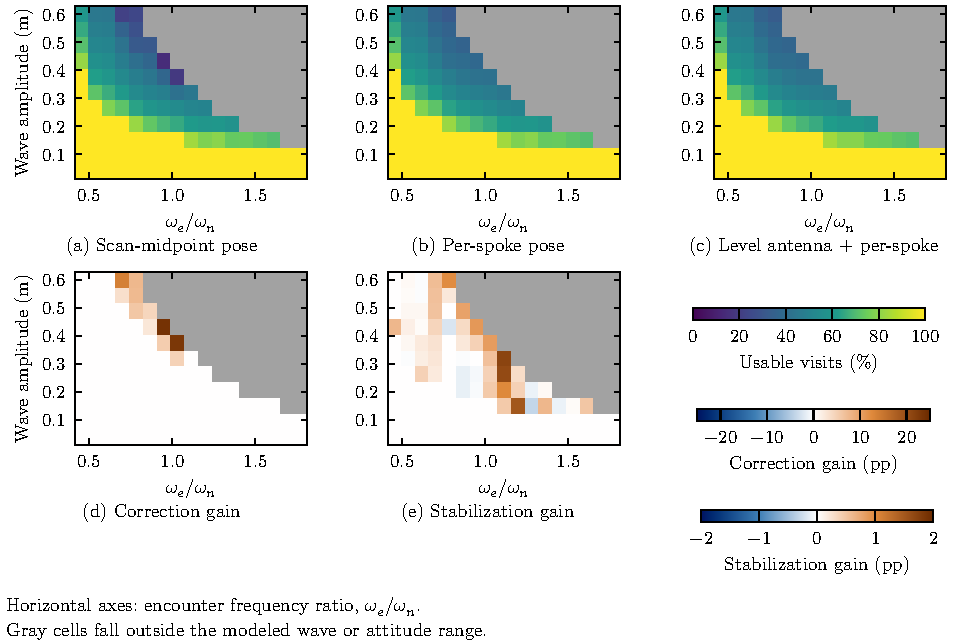
\includegraphics[width=\textwidth]{figures/operating/operating-map.pdf}
  \caption{Screened operating map of regular-wave conditions. Panels (a)--(c) report the usable fraction over 6,144 scheduled visits per cell for each method. Panels (d) and (e) give the paired gains from pose correction and level pointing in percentage points on different labeled scales. The gray cells fall outside the wave or attitude limits.}
  \label{fig:operating-map}
\end{figure*}



\subsection{Operating limits}

All three mapped arms gave 100\% usability in 50 of 111 forward, zero-yaw regular-wave cells (Fig.~\ref{fig:operating-map}). Timing correction recovered positions in 11 cells. The maximum gain was $23.76\pm0.41$ points at 0.3325 Hz and 0.432 m amplitude. Of 6,144 visits, 61.95\% had no echo, 23.76\% yielded an echo outside tolerance with the midpoint pose, and 14.29\% yielded a usable position. Correcting both pose components raised usability to 38.05\% and reduced the 95th percentile of consecutive misses from 22 visits to four.

Leveling after registration changed usability by $-0.31\pm0.12$ to $+1.71\pm0.41$ points across the grid. The tilted antenna sometimes pointed closer to the buoy. At 0.4475 Hz and 0.152 m, leveling lost 19 near-threshold echoes. In the separate reference neighborhood at fixed 0.150 m amplitude, the gain fell from 8.97 to 7.03 to zero points at 0.345, 0.350, and 0.355 Hz. Intervals describe individual cells and exclude uncertainty from selecting a maximum.

We multiplied the acquisition and position-pass fractions over all scheduled visits to test independence. The product matched midpoint usability in 100 of 111 cells, underestimated it in seven, and overestimated it in four by up to 3.75 percentage points. At 0.30375 Hz and 0.488 m, it raised the estimated registration gain from 4.39 to 13.51 percentage points. Resampling whole phase records gave a 95\% overstatement interval of 9.02--9.20 points. Both noiseless spoke-time arms factorized exactly because registration always passed.

\subsection{Interaction between pointing and registration}

Table~\ref{tab:four-arms} compares all four combinations. To isolate stand-alone interventions, we also mapped level-pointed echoes with the midpoint origin and level axes. Ranking the stand-alone gains changed the preferred first intervention in five of 111 cells relative to ranking registration against the additional gain of leveling after registration. In each, leveling led by 0.31--0.85 percentage points. At 0.36125 Hz and 0.376 m, leveling alone gained 24.01 points, recovering 1,421 positions from echoes both policies acquired and 54 from newly acquired echoes. With spoke-time registration already applied, leveling recovered those 54 echoes and lost two, yielding 0.85 points. The interaction was $-23.16$ percentage points because either intervention corrected much of the same mapping error. At 90-degree bearing in the largest registration-gain wave, leveling with the midpoint origin instead moved 692 acquired positions outside tolerance and recovered three new echoes.

\begin{table}[tb]
\caption{Usable positions out of 6,144 scheduled visits per wave. Columns cross antenna pointing with registration time.}\label{tab:four-arms}
\centering\small
\begin{tabular}{@{}lrrrr@{}}
\toprule
 & \multicolumn{2}{c}{Body-fixed} & \multicolumn{2}{c}{Level}\\
\cmidrule(lr){2-3}\cmidrule(l){4-5}
Wave (Hz, m) & Midpoint & Spoke & Midpoint & Spoke \\
\midrule
0.3500, 0.150 & 5,712 & 5,712 & 6,144 & 6,144 \\
0.3325, 0.432 & 878 & 2,338 & 2,091 & 2,392 \\
0.36125, 0.376 & 1,163 & 2,586 & 2,638 & 2,638 \\
\bottomrule
\end{tabular}
\end{table}


\subsection{Which pose component recovers an echo's position?}
At 0.3325 Hz and 0.432 m, midpoint origin and attitude gave 878 usable positions from 2,338 acquired echoes. Updating only the origin gave 1,730, only attitude gave 2,081, and both gave 2,338. The prescribed surge has the opposite sign to the free-particle horizontal orbit under our phase convention. With the original surge, none, and reversed surge, the interactions were $-18.86$, $-9.34$, and $-16.47$ points at this wave and $-23.16$, $-12.58$, and $-21.91$ points at 0.36125 Hz and 0.376 m. The reference wave gave zero interaction for every sign. The original surge mismatch reached 0.48 m against a 0.50 m tolerance. Halving surge reduced the registration gain from 23.76 to 11.59 points. Removing roll gave 4.13 points. Adding sinusoidal yaw of $1^\circ$ increased the gain to 33.35 points. Isolating bearing at an imposed 625 ms delay gave zero registration gain abeam and 32.11 points astern. With the physical crossing times below, the same bearings gave 24.28 and 24.58 points. The position test acts on the coupled motion and viewing direction.

At this forward target with 0.25 m range noise, raising the bearing standard deviation from $0.25^\circ$ to $1^\circ$ cut registration gain from 10.32 to 2.26 points.

\subsection{Common beam crossings with heading retained}

We set the rotating beam to $-90^\circ$ at each scan midpoint and solved for its crossing of the moving target bearing. The four arms shared these body-beam times. At the scan seam the pose delay wrapped to the neighboring midpoint. We tested eight bearings from $-90^\circ$ to $180^\circ$ with and without $1^\circ$ sinusoidal yaw at the wave frequency. Level pointing retained yaw at the assigned pose time.

At zero yaw the original forward counts were recovered with the quarter-scan clock. Solving the crossing changed the forward interaction from $-23.16$ to $-23.19$ points at 0.36125 Hz and 0.376 m. With yaw retained, the stand-alone leveling gain fell from 24.06 to $-1.86$ points, and the interaction became $+2.73$ points. At bearings $(-90,0,45,89.5,90,90.5,135,180)^\circ$, zero-yaw crossing interactions in this wave were $(0,-23.19,-0.47,-7.91,-2.70,-4.25,+13.33,-23.08)$ points. At $135^\circ$ leveling alone lost 13.33 points, reversing the interaction even without yaw. Adding yaw cut the forward body-midpoint usable count from 1,161 to 197 of 6,144 and raised the pose-only gain from 23.19 to 38.43 points. In the reference wave the count fell from 5,712 to 696 and timing alone gained 82.03 points, while the interaction reached $+6.64$ points. Crossing shifts were at most 10.8 ms. The stale heading can therefore govern the benefit of a level mount even when the spoke time changes little.


\subsection{Does the path model change the pointing decision?}
At the reference wave, diffraction gave 92.97\% acquisition for body pointing and 100\% for level pointing. A direct-ray visibility gate gave 100\% for both. The simulated 7.03-point benefit arose on geometrically clear rays near a crest. Adding Gaussian fluctuations to power margin reduced the expected gain to 2.41 points at 1 dB standard deviation and 1.37 at 3 dB. At the strongest registration cell diffraction gave 38.05\% for body pointing, 38.93\% for level pointing, and 38.98\% with zero angular loss. A clear-ray gate gave 42.27\% for every policy. Consequently even ideal steering recovers fewer than one extra visit per hundred there under the effective-edge model.

We also replaced the effective edge with one edge per local water crest. The Deygout construction selects the largest Fresnel--Kirchhoff parameter on each subpath, splits at that crest, and sums the resulting losses \cite{DeMinco2025Diffraction}. At the reference wave, restricting the single edge to a crest reduced the leveling gain from 7.03 to 3.13 percentage points. Including the remaining crests reduced it to 0.39 points. In the wave with the largest original registration gain, the multiple-edge model gave 10.12 points from registration and another 4.72 points from leveling. The separated-crest model changed the gain magnitudes and preserved the intervention ordering in these two waves.

As a separate sensitivity, we replaced diffraction with a direct ray and a specular ray from a horizontal plane at the buoy's instantaneous water level. Each ray used its departure angle. Reciprocal return power followed the fourth power of the summed field magnitude \cite{Galati2020Multipath}. Sweeping reflection magnitudes from zero to one and phases in $5^\circ$ steps gave leveling gains after spoke-time registration of zero to 32.42 points at the reference and zero to 32.49 at the largest-interaction wave. Both ranges collapsed to zero at $180^\circ$ reflection phase.


\subsection{Timing and precision requirements}
To compare against a system that already timestamps each spoke, we repeated all 111 grid cells with common Gaussian range and bearing errors (standard deviations 0.25 m and $0.25^\circ$). Median gains from replacing pose ages of 50, 100, 200, and 625 ms with exact timing were 0.07, 0.16, 0.49, and 3.37 percentage points, respectively. The corresponding maxima were 0.62, 1.03, 3.11, and 12.30 points. These are equally weighted grid summaries. Delay is a controlled input and requires measurement on the installed system.

At the strongest registration cell, delaying the assigned pose by up to 0.40 s at the sampled delays left all 2,338 acquired echoes within tolerance. At 0.50 s, 627 fell outside, and at 0.625 s the delay reproduced all 1,460 midpoint failures. For the $8.28^\circ$ peak pitch, Eq.~\eqref{eq:pose-delay} gives peak pitch mismatches of $6.7^\circ$ and $8.3^\circ$ at 0.40 and 0.50 s, respectively. The counting threshold depends on the phase of the echoes that survive.

At the reference wave the gain from leveling after timing correction was 1.56, 7.03, and 0.00 points at 5, 10, and 15 dB clear margin. Redistributing the reference elevation variance over seven frequencies reduced it to $0.59\pm0.19$ points and left no registration gain. The corresponding frequency ratios are $(0.72,0.83,0.92,1,1.08,1.18,1.29)$ with variance fractions $(0.08,0.13,0.19,0.23,0.19,0.12,0.06)$.


\subsection{Sensitivity to quadratic pitch damping}
\label{sec:nonlinear-pitch}

The largest linear-model registration gain occurs near pitch resonance, where high angular speed also amplifies rate-dependent damping. Suzuki et al. fitted linear and quadratic pitch damping to free-decay tests on a floating wind turbine platform \cite{Suzuki2021Floater}. We adopt the form of that damping law for a sensitivity study with prescribed coefficients. The pitch equation retains the original wave-slope excitation and adds a damping torque proportional to angular speed squared. After dividing by the effective pitch inertia, it becomes
\begin{equation}
  \ddot\theta+d_1\dot\theta+d_2|\dot\theta|\dot\theta+\omega_n^2\theta
  =-\omega_n^2 G\,\partial_x\eta(\mathbf{0},t),
  \label{eq:quadratic-pitch}
\end{equation}
where $d_1=2\zeta\omega_n$. The two damping terms dissipate mechanical power per unit effective inertia at the rate $d_1\dot\theta^2+d_2|\dot\theta|^3$. To prescribe the strength of the nonlinear term, we use $\chi=d_2 v_{\mathrm{ref}}/d_1$, the ratio of quadratic to linear damping torque magnitudes at $v_{\mathrm{ref}}=0.123$ rad/s, the peak pitch rate of the linear mode at the reference wave. We test $\chi=0$, $0.25$, $0.50$, and $1.00$, spanning the linear baseline through equal damping contributions at that speed.

We integrate Eq.~\eqref{eq:quadratic-pitch} directly from rest and use the cycle following 60 forcing periods to evaluate the phase-shifted pitch at every spoke and midpoint. The new pitch changes both the pointing angle and the rotated antenna lever arm, so we recompute the diffraction path and mapping at each visit. We pair the same incident waves, roll, surge, and heave across damping levels, with 192 visits in each of 32 initial phases. At $\chi=0$, direct integration reproduces the acquisition and registration decisions of the closed-form solution in all seven tested wave conditions. Extending spin-up to 80 cycles and halving the maximum integration step changes pitch by at most $6.6\times10^{-12}$ rad and leaves every visit classification identical. Cycle-integrated forcing work balances dissipation and the change in mechanical energy to a relative residual below $4.4\times10^{-14}$.

\begin{figure*}[t]
\centering
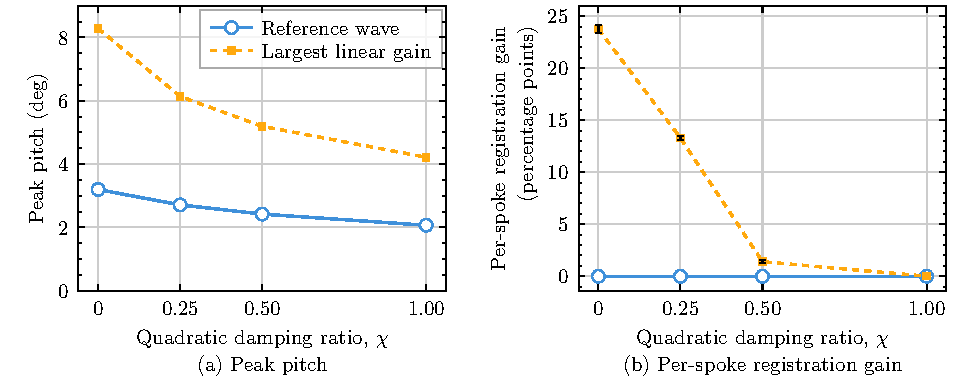
\includegraphics[width=.95\textwidth]{figures/operating/nonlinear-pitch.pdf}
\caption{Peak pitch and registration gain as the quadratic pitch damping increases. The reference wave is 0.350 Hz and 0.150 m. The largest-gain cell of the linear map is 0.3325 Hz and 0.432 m. Gain measures the increase in usable visits over midpoint registration. Error bars give paired 95\% intervals over initial wave phases.}
\label{fig:nonlinear-pitch}
\end{figure*}

At the largest-gain cell, the quadratic term dissipates 51.4\% of the cycle's input work at $\chi=1$. The fundamental pitch lag rises from $71.1^\circ$ to $81.0^\circ$ and the third harmonic reaches 0.81\% of the fundamental amplitude. As peak pitch falls from $8.28^\circ$ to $4.21^\circ$, the scan-midpoint estimate satisfies the position tolerance for progressively more of the acquired echoes. Figure~\ref{fig:nonlinear-pitch} shows the per-spoke registration gain falling from 23.76 to 13.30 to 1.40 to 0.00 percentage points, even as body-pointed acquisition rises from 38.05\% to 38.57\%. The 0.30375 Hz neighbor at fixed amplitude, the 0.376 m neighbor at fixed frequency, and the pilot wave all reach zero registration gain at $\chi=0.25$.

At the reference wave, all acquired echoes meet the position tolerance throughout the damping sweep. Lower pitch increases body-pointed acquisition from 92.97\% to 95.31\% and reduces the additional gain from leveling by $2.34\pm1.72$ percentage points at $\chi=1$ relative to $\chi=0$, using the paired phase interval. The neighboring 0.345 and 0.355 Hz waves also retain zero registration gain at the reference amplitude. These cases show that near resonance, the damping law affects whether midpoint registration crosses the position tolerance, while wave obstruction still limits acquisition in the larger-amplitude conditions.

\subsection{Sensitivity to second-order wave shape}
\label{sec:crest-sensitivity}

Changing crest shape can move an echo across the power threshold even when the vessel follows the same trajectory. To isolate this effect, we paired each linear regular wave with the second-order deep-water Stokes surface \cite{Chen2018StokesHarmonics}. For fundamental phase $\chi=\mathbf{k}\cdot\mathbf{x}-\omega t+\psi$, the bound harmonic gives
\begin{equation}
 \eta_2=a\cos\chi+\tfrac12 ka^2\cos(2\chi).
\end{equation}
We used $\eta_2$ at the buoy's fixed horizontal location and along the instantaneous ray, retaining the same hull motion and visit times. The surface gradient magnitude is bounded by $ka+(ka)^2$. At the largest linear registration-gain cell, the peak slope rises from $ka=0.192$ to $0.205$, so the perturbed case probes the edge of the nominal $ka\le0.20$ screen.

At the reference point, the 5.55 mm harmonic reduces the unstabilized usable fraction from $92.97\%$ to $91.02\%$. The level-pointed fraction stays at $100\%$. At the largest linear registration-gain cell, the 41.5 mm harmonic reduces the number of body-pointed echoes from 2,338 to 1,960 and changes the number meeting tolerance with the midpoint pose from 878 to 879. The per-spoke registration gain consequently falls from 23.76 to 17.59 percentage points. In the pilot record, the number of echoes acquired drops from 96 to 72 of 192 visits, while per-spoke correction still recovers 48 out-of-tolerance positions. Refining the ray sampling from 601 to 1,201 points changes two level-pointed classifications in the strongest cell and none in the other comparisons. The relative prevalence of the two failure modes thus depends on the modeled crest clearance and buoy elevation.

\subsection{Directional spreading at fixed wave spectrum}

For a separate symmetric seven-mode spectrum, we paired long-crested and directionally spread seas with identical frequencies, amplitudes, and 64 sets of phases over 480 s. The seven frequency ratios above used variance fractions $(.07,.125,.19,.23,.19,.125,.07)$ and heading offsets $(-40,27,-15,0,15,-27,40)^\circ$. The 0.350 Hz reference retained its 0.150 m equivalent regular-wave amplitude. At 0.3325 Hz, the slope limit of 0.20 reduced the equivalent amplitude from 0.432 to 0.168 m in both seas. Across the cases, pitch and roll were bounded by $6.74^\circ$ and $1.98^\circ$. Registration gained zero usable visits. Spreading changed the leveling gain from 0.58 to 0.29 percentage points at the reference and from 0.08 to 0.32 at 0.3325 Hz. The 95th-percentile longest update gap stayed at 12.5 s at the reference and fell from 12.5 to 10.0 s at 0.3325 Hz.

\subsection{Holding the last fix with orbital buoy motion}
The buoy moved horizontally by $-a\sin\varphi$ along wave travel, where $\varphi$ is the wave phase at its mean position. A zero-order hold retained the last acquired finite fix and we scored that estimate against contemporaneous truth at every visit. Visits before the first fix counted as unusable. With range and bearing noise standard deviations of 0.25~m and $0.25^\circ$, midpoint and spoke-time usability were 14.3\% and 24.5\% for fresh fixes and 37.7\% and 50.8\% with holding at the strongest-gain condition. At the reference condition, the corresponding fractions were 56.3\% and 59.9\% for fresh fixes and 60.7\% and 65.2\% with holding.

\subsection{Revisit phase and elapsed outage duration}

With a uniform starting phase, every independently scheduled visit samples the same marginal wave-phase distribution. Expected usability is therefore independent of the clock in a regular wave with exact spoke registration and fixed margin. The sequence of failures still depends on the phase increment. For a 0.42 Hz wave giving $3^\circ$ peak pitch we simulated 256 starting phases per schedule over 480 s. The perturbed schedules draw each interval uniformly and independently within the stated percentage of the nominal period. Gaps intersecting a record boundary contribute their observed duration. An entirely missed record counts as 480 s.

At fixed 0.42 Hz, mean usability stayed within 64.6--65.3\%. Yet increasing the constant scan period from 1.25 to 2.50 s raised the 95th-percentile longest gap from 2.5 to 20.0 s. At exact lock (2.381 s), 90 of 256 records produced no update. Independent uniform interval perturbations of $\pm10\%$ reduced the exact-lock gap percentile from 480 to 112.5 s but lengthened it from 20.0 to 44.0 s for the 2.50 s clock. Thus jitter can increase or decrease the longest gaps.

\subsection{Selecting a fixed rotation speed}

We selected among 24, 36, and 48 revolutions per minute by minimizing the predicted 95th-percentile longest update gap. The predictor used encounter frequency rounded to the nearest bin of a 120 s record and a visible sector fixed at half the wave cycle. Ties favored the fastest speed. The diffraction model scored each speed over 480 s with 256 shared random phases in each of 40 wave conditions outside the original grid. We compared a constant 10 dB margin with a dwell sensitivity of $10+10\log_{10}(T/2.5\,\mathrm{s})$ dB for rotation period $T$, representing coherent integration at constant pulse rate.

The rule chose 48 revolutions per minute in 38 conditions. Both switches to 36 lengthened the gap percentile, by up to 17.92 s at constant margin and 44.58 s with dwell scaling. Relative to fixed 24, the median improvement across conditions was 3.75 s under either margin. The best speed chosen after scoring improved on fixed 48 in four and two conditions, respectively. Fixed 48 matched or outperformed the frequency-only rule throughout the grid.


\section{Design implications}
Two measurements determine whether the modeled gains justify an intervention. For registration, replay identical echoes with their original and corrected timestamps and compare both against an independently tracked buoy. Measure the residual range, bearing, and height errors after correction. At 100 m, $0.29^\circ$ of bearing error alone consumes the 0.50 m budget. The manufacturer specifies bearing accuracy of $\pm1^\circ$. That specification does not establish the precision of the buoy centroid. A measured latency well below the simulated failure threshold or a residual exceeding tolerance can eliminate the return on a timestamp change.

For pointing, log all attempted visits together with calibrated echo and clutter powers, antenna attitude, and commanded and attained angles. Interleaved pointing policies or synchronized antennas can separate changes in pointing from changes in sea state. A reflected ray in the still-water reference geometry differs in length from the direct ray by about 0.29 wavelengths. Interference, clutter, and target scattering can therefore change the margin distribution that determines whether leveling recovers any visits. For track continuity, compare scanners over equal durations and retain intervals with no update. Compare any adaptive clock against the fastest available fixed setting with its measured dwell-dependent sensitivity.

\section{Conclusion}
The stand-alone hardware and software retrofits corrected many of the same positions. Adding their individual gains would double count those recoveries. In two 4 Hz field clips the measured change in median repeatability was at most 6 mm. Across the noisy simulation grid, reducing an existing 50 ms delay yielded less than one additional usable position per hundred visits in every cell. At the largest noiseless midpoint gain, quadratic pitch damping reduced the registration gain from 23.76 to 1.40 points at $\chi=0.50$. At the smaller reference wave the apparent pointing benefit disappeared under an alternative propagation law. In the clock experiment the fastest fixed speed matched or beat the frequency-based rule in every held-out case. The resulting design priorities depend on the residual error of real echoes, the fraction of visits near the detector threshold, and the longest gap the tracker can tolerate.

\section*{Data and code availability}
The simulation, per-realization counts, model checks, and scripts for the sensitivity studies accompany the manuscript in the EMCH 574 project directory of the author's repository \cite{Vaught2026RadarStudy}. The scripts reproduce the tables and plotting inputs from the specified configurations.

\bibliographystyle{asmeconf}
\bibliography{operating-refs,references,review-additions,nonlinear-model}
\end{document}
